\section{Durchführung}
\label{sec:Durchführung}

Zur Messung des Brechungsindex wird ein Prismenspektralapperat wie in Abbildung \ref{fig:j3} benutzt.
\begin{figure}
  \centering
  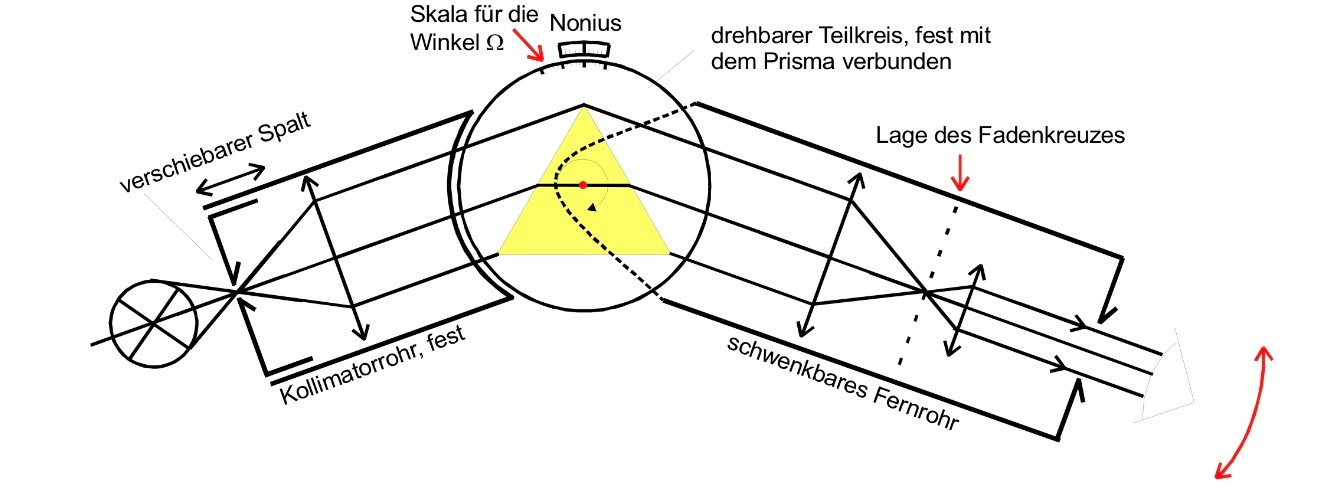
\includegraphics[height=6cm]{data/j3.jpg}
  \caption{Skizze eines Prismenspektralapperats. \cite{sample}}
  \label{fig:j3}
\end{figure}
Mit Hilfe des Snelliusschen Brechungsgesetztes kann aus den Winkelbeziehungen im Prisma (siehe Abb. \ref{fig:j4}) der Brechungsindex bestimmt werden.
\begin{figure}
  \centering
  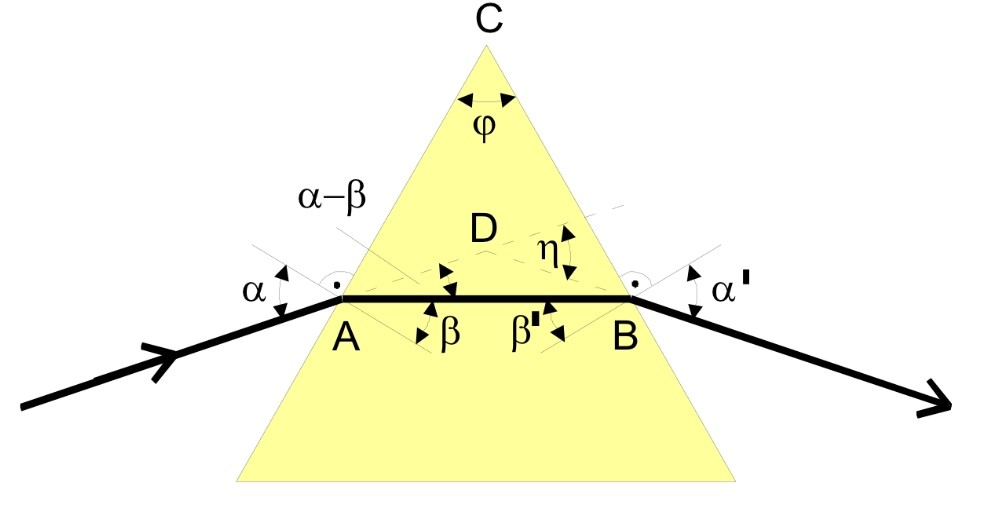
\includegraphics[height=5cm]{data/j4.jpg}
  \caption{Symmetrischer Strahlengang durch ein Prisma. \cite{sample}}
  \label{fig:j4}
\end{figure}
\begin{equation}
  n = \frac{\sin(\alpha)}{\cos(\beta)}
\end{equation}
Bei einem symmetrischen Strahlengang durch das Prisma ($\alpha = \alpha'$ und $\beta = \beta'$) ergeben sich für die benötigenten Winkel folgende Beziehungen:
\begin{align}
  \alpha &= \frac{\eta + \phi}{2} \\
  \beta &= \frac{\phi}{2}
\end{align}
Die Winkel $\eta$ und $\phi$ können über zwei verschiedene Methoden bestimmt werden.
Die Messung von $\phi$ erfolgt indirekt über die Messung von $\phi_l$ und $\phi_r$ wie in Abbildung \ref{fig:j5} zu sehen.
\begin{figure}
  \centering
  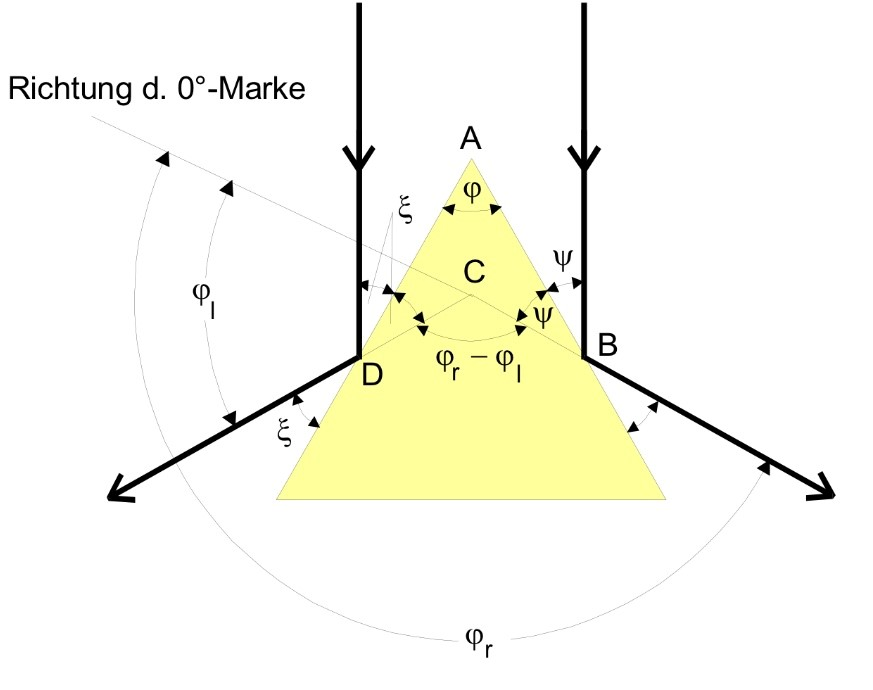
\includegraphics[height=6cm]{data/j5.jpg}
  \caption{Bestimmung des Winkels $\phi$. \cite{sample}}
  \label{fig:j5}
\end{figure}
Dabei handelt es sich um die Reflexionswinkel, die auftreten, wenn das Licht der Hg-Cb-Lampe parrallel zur Spitze auf die brechenden Kanten fällt.
\begin{equation}
  \phi = \frac{1}{2} (\phi_r - \phi_l)
\end{equation}
Für die Bestimmung von $\eta$ wird das Prisma so gedreht, dass reflektierter und gebrochener Strahl in Deckung sind.
Der Winkel am Goniometer wird abgelesen und die Messung für die spiegelsymmetrische Stellung wiederholt (siehe Abb. \ref{fig:j6}).
\begin{figure}
  \centering
  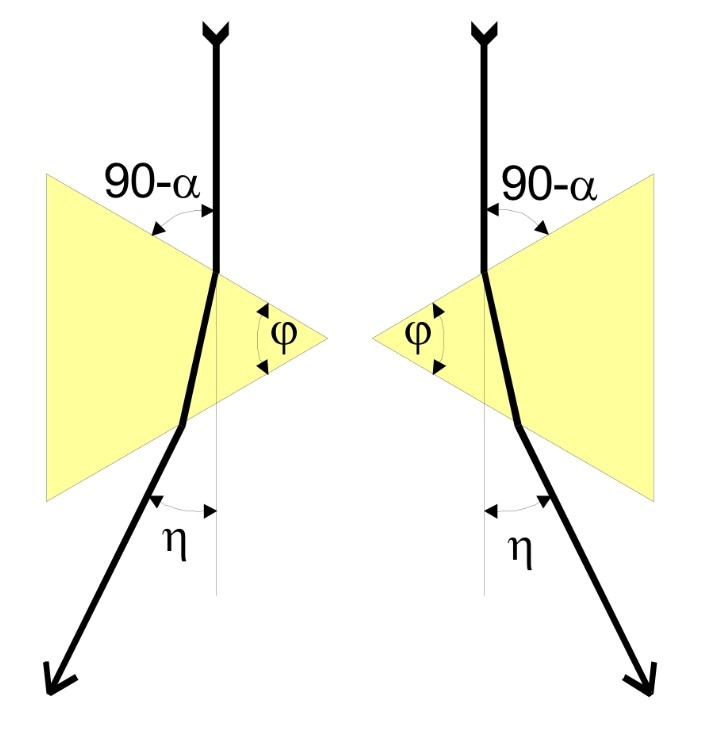
\includegraphics[height=6cm]{data/j6.jpg}
  \caption{Bestimmung des Winkels $\eta$. \cite{sample}}
  \label{fig:j6}
\end{figure}
$\eta$ berechnet sich dann folgendermaßen:
\begin{equation}
  \eta = 180 - (\eta_r - \eta_l)
\end{equation}
